\chapter{Anytime Approximate Formal Feature Attribution}\label{chap:marco}


This chapter is based on:
\begin{itemize}
	\item Jinqiang Yu, Graham Farr, Alexey Ignatiev, and Peter J. Stuckey. Anytime Approximate Formal
Feature Attribution. \emph{arXiv preprint arXiv:2312.06973,} 2023.
\end{itemize}

\autoref{chap:ffa} provides a clear and crisp definition of FFA, but its computation presents
challenges,
since determining whether a feature has a non-zero attribution is as
least as hard as determining its relevance.
%
In \autoref{chap:ffa}, we demonstrate that FFA computation can be efficiently achieved 
by leveraging the hitting set duality between AXp's and CXp's.
%
While attempting to enumerate CXp's, a side effect of the algorithm is 
the discovery of AXp's. 
%
Indeed, the algorithm typically identifies numerous AXp's before encountering the first CXp.
%
In this case, the AXp's at the beginning are ensured to be diverse, as they must be broad in scope
to guarantee that the CXp is large enough to hit all relevant AXp's for exact FFA.
%
Therefore, collecting AXp's as side effects of CXp enumeration proves effective in the 
initial stages of the enumeration process.
%
However, as we collect an increasing number of AXp's as side effects, we eventually 
reach some point where significantly more CXp's are generated than AXp's.
%
Experimental results indicate that if we aim to enumerate all AXp's, it is preferable not to 
depend on the side effect behavior, but rather to directly enumerate AXp's.
%
This presents a dilemma: for fast and accurate approximations of FFA, we enumerate CXp's and
generate AXp's as a side effect, while to produce exact FFA, we compute all AXp's, and it is more 
advantageous to directly enumerate them.
%
In this chapter, we introduce an anytime method to produce approximate FFA,
where we initially enumerate CXp's and then switch to AXp enumeration dynamically 
when the rate of AXp discovery through CXp enumeration decrease.
%
Thus, we can quickly obtain accurate approximations while also accelerating the process of 
arriving at the complete set of AXp's compared to pure CXp enumeration.
%
The second contribution of this work involves exploring this alternative approach 
and demonstrating that even with a(n) (in)complete set of CXp's provided, 
determining FFA remains computationally challenging, as it is \#P-hard even when 
all CXp's are of size two.


%As direct CXp enumeration is feasible to do without the need to resort
%to the hitting set duality~\cite{msi-aaai22}, one may want to estimate
%FFA by first enumerating CXp's.
%

%The second contribution of this paper is to investigate this
%alternative approach and to show that even if a(n) (in)complete set of
%CXp's is given, determining FFA is computationally expensive being
%\#P-hard even if all CXp's are of size two.

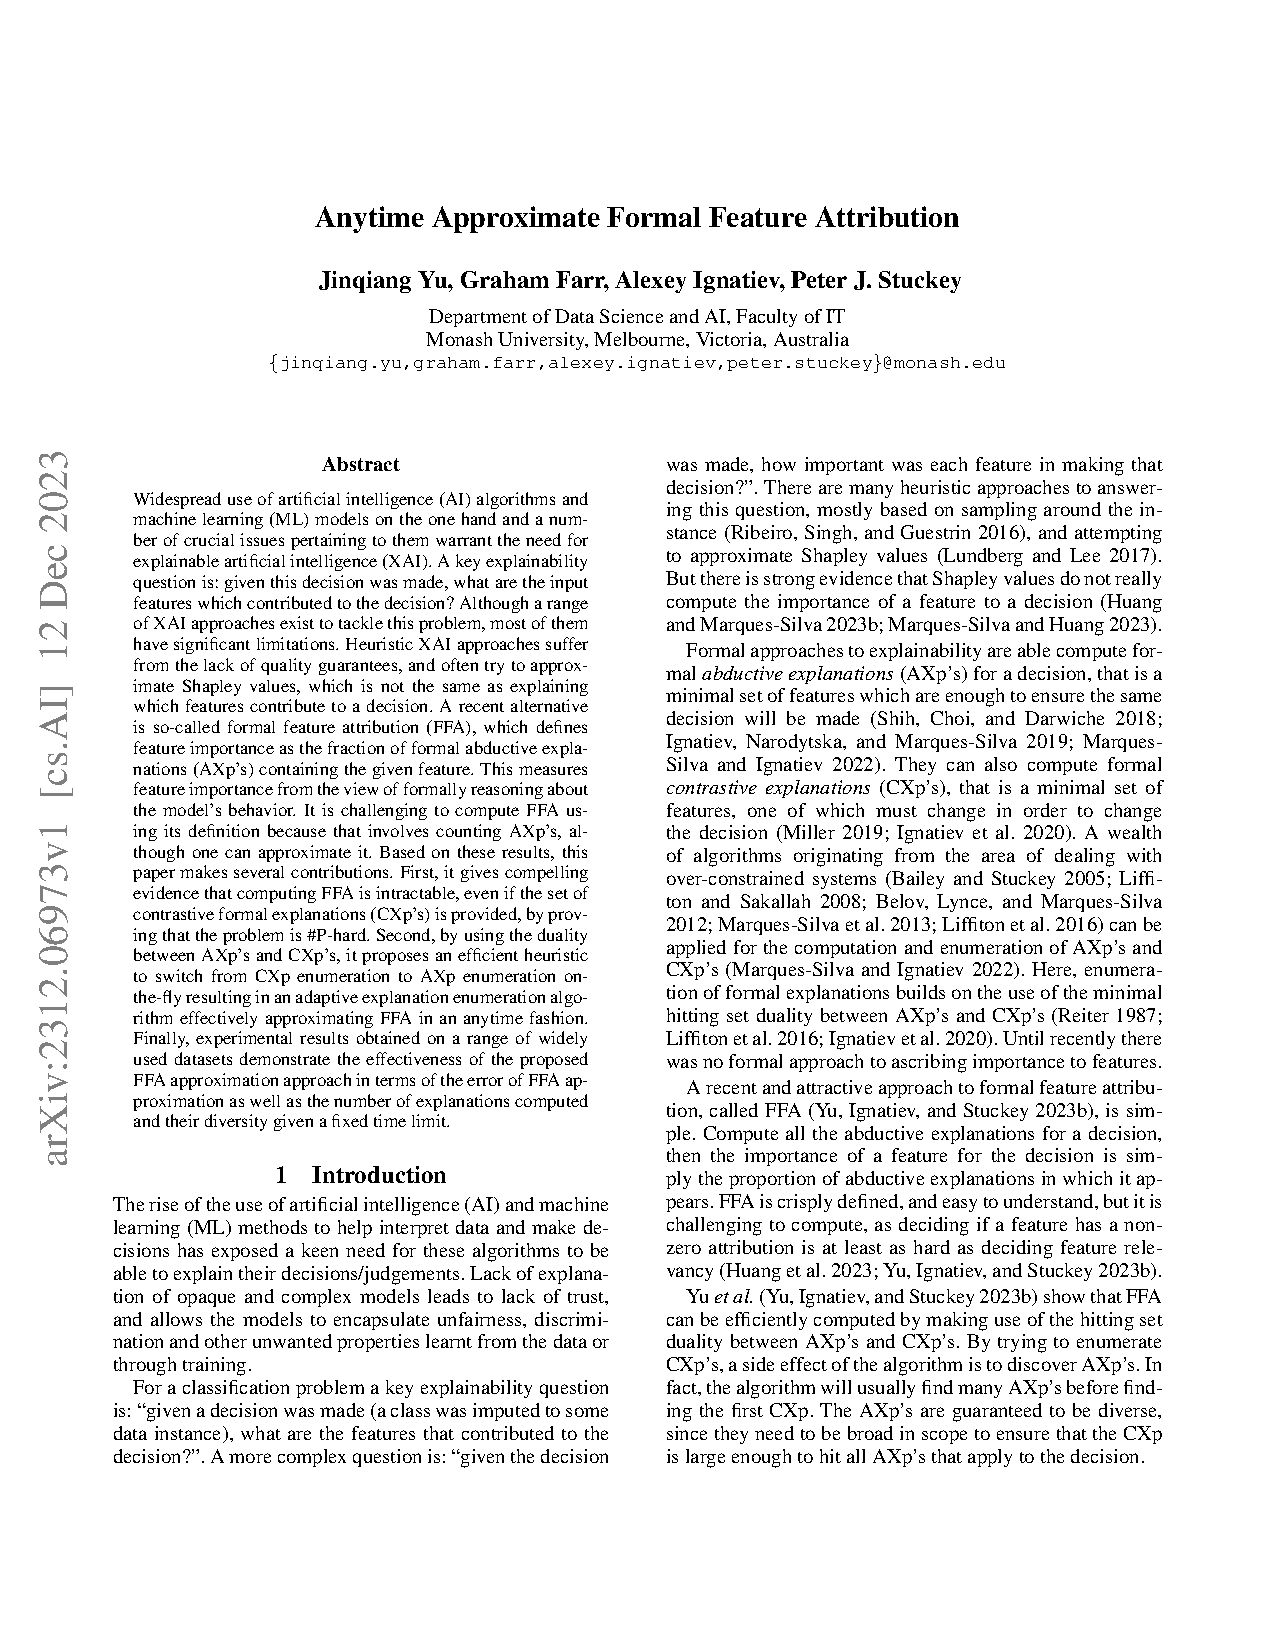
\includepdf[pages=-, offset=75 -75]{papers/marco.pdf}
